% ----------------------------------------------------
% Tutorial
% ----------------------------------------------------
\documentclass[class=report,11pt,crop=false]{standalone}
% Page geometry
\usepackage[a4paper,margin=20mm,top=25mm,bottom=25mm]{geometry}

\newcommand{\tabitem}{~~\llap{\textbullet}~~}
% Font choice
\usepackage{lmodern}

\usepackage{lipsum}

% Use IEEE bibliography style
\bibliographystyle{IEEEtran}

% Line spacing
\usepackage{setspace}
\setstretch{1.20}

% Ensure UTF8 encoding
\usepackage[utf8]{inputenc}

% Language standard (not too important)
\usepackage[english]{babel}

% Skip a line in between paragraphs
\usepackage{parskip}

% For the creation of dummy text
\usepackage{blindtext}

% Math
\usepackage{amsmath}

% Header & Footer stuff
\usepackage{fancyhdr}
\pagestyle{fancy}
\fancyhead{}
\fancyhead[R]{\nouppercase{\rightmark}}
\fancyfoot{}
\fancyfoot[C]{\thepage}
\renewcommand{\headrulewidth}{0.0pt}
\renewcommand{\footrulewidth}{0.0pt}
\setlength{\headheight}{13.6pt}

% Epigraphs
\usepackage{epigraph}
\setlength\epigraphrule{0pt}
\setlength{\epigraphwidth}{0.65\textwidth}

% Colour
\usepackage{color}
\usepackage[usenames,dvipsnames]{xcolor}

% Hyperlinks & References
\usepackage{hyperref}
\definecolor{linkColour}{RGB}{77,71,179}
\hypersetup{
    colorlinks=true,
    linkcolor=linkColour,
    filecolor=linkColour,
    urlcolor=linkColour,
    citecolor=linkColour,
}
\urlstyle{same}

% Automatically correct front-side quotes
\usepackage[autostyle=false, style=ukenglish]{csquotes}
\MakeOuterQuote{"}

% Graphics
\usepackage{graphicx}
\graphicspath{{Images/}{../Images/}}
\usepackage{makecell}
\usepackage{transparent}

% SI units
\usepackage{siunitx}

% Microtype goodness
\usepackage{microtype}

% Listings
\usepackage[T1]{fontenc}
\usepackage{listings}
\usepackage[scaled=0.8]{DejaVuSansMono}

% Custom colours for listings
\definecolor{backgroundColour}{RGB}{250,250,250}
\definecolor{commentColour}{RGB}{73, 175, 102}
\definecolor{identifierColour}{RGB}{196, 19, 66}
\definecolor{stringColour}{RGB}{252, 156, 30}
\definecolor{keywordColour}{RGB}{50, 38, 224}
\definecolor{lineNumbersColour}{RGB}{127,127,127}
\lstset{
  language=Matlab,
  captionpos=b,
  aboveskip=15pt,belowskip=10pt,
  backgroundcolor=\color{backgroundColour},
  basicstyle=\ttfamily,%\footnotesize,        % the size of the fonts that are used for the code
  breakatwhitespace=false,         % sets if automatic breaks should only happen at whitespace
  breaklines=true,                 % sets automatic line breaking
  postbreak=\mbox{\textcolor{red}{$\hookrightarrow$}\space},
  commentstyle=\color{commentColour},    % comment style
  identifierstyle=\color{identifierColour},
  stringstyle=\color{stringColour},
   keywordstyle=\color{keywordColour},       % keyword style
  %escapeinside={\%*}{*)},          % if you want to add LaTeX within your code
  extendedchars=true,              % lets you use non-ASCII characters; for 8-bits encodings only, does not work with UTF-8
  frame=single,	                   % adds a frame around the code
  keepspaces=true,                 % keeps spaces in text, useful for keeping indentation of code (possibly needs columns=flexible)
  morekeywords={*,...},            % if you want to add more keywords to the set
  numbers=left,                    % where to put the line-numbers; possible values are (none, left, right)
  numbersep=5pt,                   % how far the line-numbers are from the code
  numberstyle=\tiny\color{lineNumbersColour}, % the style that is used for the line-numbers
  rulecolor=\color{black},         % if not set, the frame-color may be changed on line-breaks within not-black text (e.g. comments (green here))
  showspaces=false,                % show spaces everywhere adding particular underscores; it overrides 'showstringspaces'
  showstringspaces=false,          % underline spaces within strings only
  showtabs=false,                  % show tabs within strings adding particular underscores
  stepnumber=1,                    % the step between two line-numbers. If it's 1, each line will be numbered
  tabsize=2,	                   % sets default tabsize to 2 spaces
  %title=\lstname                   % show the filename of files included with \lstinputlisting; also try caption instead of title
}

% Caption stuff
\usepackage[hypcap=true, justification=centering]{caption}
\usepackage{subcaption}

% Glossary package
% \usepackage[acronym]{glossaries}
\usepackage{glossaries-extra}
\setabbreviationstyle[acronym]{long-short}

% For Proofs & Theorems
\usepackage{amsthm}

% Maths symbols
\usepackage{amssymb}
\usepackage{mathrsfs}
\usepackage{mathtools}

% For algorithms
\usepackage[]{algorithm2e}

% Spacing stuff
\setlength{\abovecaptionskip}{5pt plus 3pt minus 2pt}
\setlength{\belowcaptionskip}{5pt plus 3pt minus 2pt}
\setlength{\textfloatsep}{10pt plus 3pt minus 2pt}
\setlength{\intextsep}{15pt plus 3pt minus 2pt}

% For aligning footnotes at bottom of page, instead of hugging text
\usepackage[bottom]{footmisc}

% Add LoF, Bib, etc. to ToC
\usepackage[nottoc]{tocbibind}

% SI
\usepackage{siunitx}

% For removing some whitespace in Chapter headings etc
\usepackage{etoolbox}
\makeatletter
\patchcmd{\@makechapterhead}{\vspace*{50\p@}}{\vspace*{-10pt}}{}{}%
\patchcmd{\@makeschapterhead}{\vspace*{50\p@}}{\vspace*{-10pt}}{}{}%
\makeatother
\begin{document}
% ----------------------------------------------------
\chapter{Tutorial}
% ----------------------------------------------------


\section{Section heading} % This is how you make a section heading
\subsection{Subsection heading} % This is how you make a subsection heading
\subsubsection{Subsubsection heading}  % This is how you make a subsubsection heading

This is a normal paragraph.

\section{How to: Figures}
\subsection{Tables}
\begin{enumerate}
    \item Let's make our first table:
        \begin{itemize}
            \item Click the "Insert Table" tool in the tool bar > Select size of table > Begin editing > Follow \href{https://www.overleaf.com/learn/latex/Tables}{this tutorial} to begin customising the table.
            \item Alternatively use \href{https://www.tablesgenerator.com}{latex table generator} to create more complicated tables
        \end{itemize}
    \item Let's populate the table:
        \begin{table}
            \centering
            \begin{tabular}{|c|cc|}
                \hline
                \textbf{See} & \textbf{this is} & \textbf{easy}\\
                \hline
                 &  & \\
                 &  & \\
                 &  & \\
                 \hline \hline
            \end{tabular}
            \caption{Caption}
            \label{tab:my_first_table}
        \end{table}
    \item Now we can reference \autoref{tab:my_first_table} or Table \ref{tab:my_first_table} from anywhere in our document! Make sure to do this because it makes your document a lot more readable and usable.
\end{enumerate}

\subsection{Images}
\begin{enumerate}
    \item Let's make add our first image:
        \begin{itemize}
            \item Click the "Insert Figure" tool in the tool bar > Select how to upload the image > Follow the instructions.
            \item Alternatively follow \href{https://www.overleaf.com/learn/latex/Inserting_Images}{this tutorial}.
        \end{itemize}
    \item Let's take a look at an example:        
            \begin{figure}
                \centering
                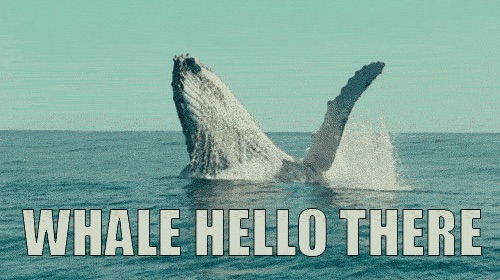
\includegraphics[width=0.5\linewidth]{EEE3088F_latex_template/Figures/whalecome.jpeg}
                \caption{My first image}
                \label{fig:my_first_image}
            \end{figure}
    \item Now we can reference \autoref{fig:my_first_image} or Figure \ref{fig:my_first_image} from anywhere in our document! Make sure to do this because it makes your document a lot more readable and usable.        
\end{enumerate}

\subsection{Other Figures}
This will likely be more useful for other courses, but LaTeX and Overleaf allow you to import other types of figures and has other cool features like allowing you to draw diagrams and plot graphs directly in LaTeX. There are plenty of resources available on how to do this, please give it a try when you have the need for it. Trust me, plotting a graph straight in LaTeX using your raw data is less time consuming than having to \textit{\textbf{repeatedly}} take screenshots in Excel. 

\section{How to: Bibliography}
\begin{enumerate}
    \item Let's make add our first citation:
        \begin{itemize}
            \item To cite sources in LaTeX you need to make use of \textbf{Bibtex}: here is \href{https://www.overleaf.com/learn/latex/Bibliography_management_in_LaTeX}{a tutorial}. 
            \item This template is already all set up to allow you to add and use citations. The template is set to the IEEE default (this is the what we will use in this and all other EEE courses). However, you will need to add any and all references you might have to the \textbf{\textit{.bib}} file (as described in the tutorial). 
                \begin{enumerate}
                    \item Navigate to the \textit{Bibliography} folder in this template > Open \textit{References.bib} > Use @... to add Bibtex references.
                    \item \textcolor{red}{\textbf{Use \href{https://bibtex.eu}{this resource} to learn all about Bibtex.}}
                \end{enumerate}
            
        \end{itemize}
    \item Let's take a look at an example:        
            \begin{center}
                This is what an in-text reference looks like in LaTeX: \cite{rick_roll}.
            \end{center}      
\end{enumerate}


\section{How to: other things}
\subsection{Cross Referencing}
This is when you make reference to chapters, sections, figures, etc from within your document. For example: 
\begin{itemize}
    \item \autoref{fig:my_first_image} or Figure \ref{fig:my_first_image}.
    \item \autoref{ch:introduction} or Chapter \ref{ch:introduction}.
\end{itemize}


\subsection{Math Equations}
Another cool thing about LaTeX is that it nicely formats your mathematical equations. \href{https://www.overleaf.com/learn/latex/Mathematical_expressions}{This tutorial} is super helpful, there are also plenty of other online resources to help you do this.





% ----------------------------------------------------
\ifstandalone
\bibliography{../Bibliography/References.bib}
\fi
\end{document}
% ----------------------------------------------------